\section{Statistical Inference}
%%%%%%%%%%%%%%%%%%%%%%%%%%%%%%%%
	\emph{Statistical Inference} is about generating and interpreting confidence intervals and setting up and testing hypotheses. Examples for questions in the field of transportation:
	\begin{itemize}
		\item Do traffic calming measures reduce speed?
		\item Did the deregulation of the airline industry impact the safety of flying?
		\item Do changeable message signs (CMS) reduce the occurrence of secondary incidents?
	\end{itemize}
\subsection{Confidence Intervals (CI)}
	Unknown parameters of the population are not known with full certainty. Working with \emph{confidence intervals} allows to quantify the degree of uncertainty around these parameters.
	\subsubsection{CI for the population mean with known standard deviation}
		When $\sigma$ is known, we can set up a confidence interval for $\mu$ using the CCT (\ref{sec:clt}). If a sample is large enough, then approximately $\bar{x}\sim N(\mu,\frac{\sigma^2}{N})$. So, for approximately normal distributed data, for $\alpha\epsilon(0,1)$, a CI with confidence level $\alpha$ is $\left[\bar{x}-z_{\frac{\alpha}{2}}\frac{\sigma}{\sqrt{n}},\,\bar{x}+z_{\frac{\alpha}{2}}\frac{\sigma}{\sqrt{n}}\right]$ with $n$ as the sample size.
		\begin{fig}[CI for the population mean with known standard deviation]{fig:ci1}{h}
			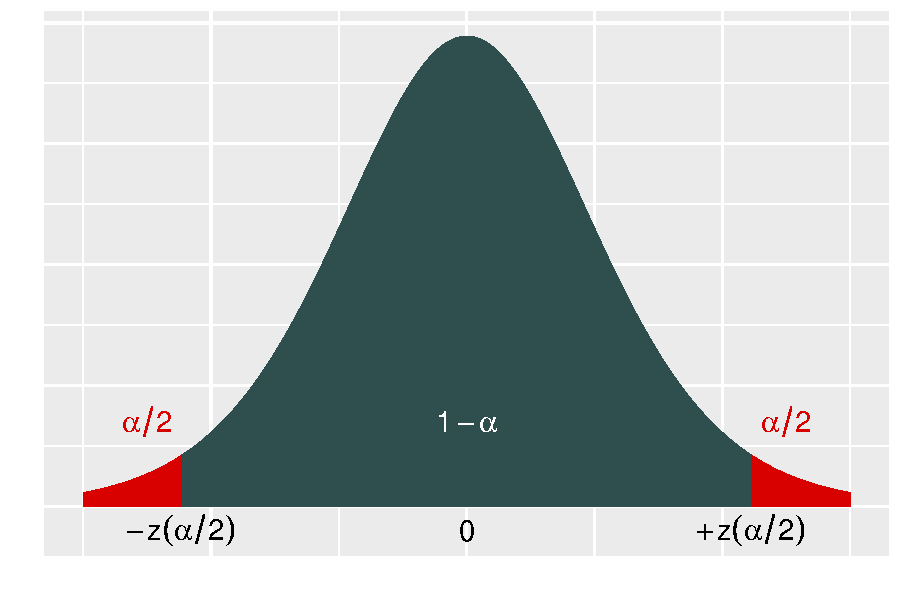
\includegraphics[width=\textwidth]{P11ci.pdf}	
			\credits{By ARAKI Satoru at Wikipedia Commons. CC BY-SA 4.0. Edited.}							
		\end{fig}
	\subsubsection{CI for the population mean with unknown standard deviation}	
		When $\sigma$ is unknown, the notation for the confidence interval changes because we will use the sample's standard error $s$ as an estimator for $\sigma$.
		\begin{equation*}
			CI(\alpha)=\left[\bar{x}-t_{\frac{\alpha}{2}}\frac{s}{\sqrt{n}},\,\bar{x}+t_{\frac{\alpha}{2}}\frac{s}{\sqrt{n}}\right]
		\end{equation*}
		\begin{fig}[CI for the population mean with unknown standard deviation]{fig:ci2}{h}
			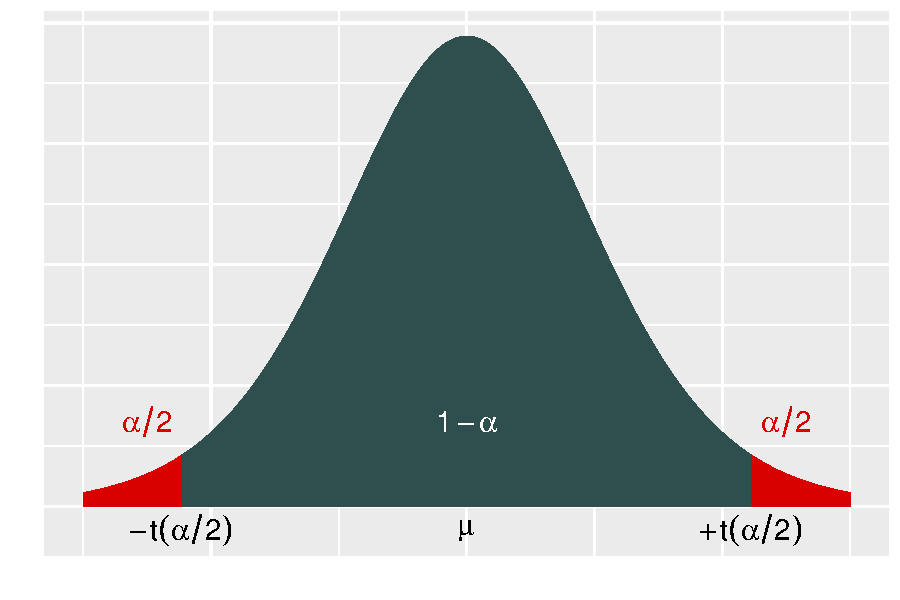
\includegraphics[width=\textwidth]{P12ci.pdf}
			\credits{By ARAKI Satoru at Wikipedia Commons. CC BY-SA 4.0. Edited.}			
		\end{fig}	
	\subsubsection{CI for a population proportion}	
		We can use a sample estimate $\hat{p}$ for a population proportion, e.g. to find out the true percentage of commuters who carpool.
		\begin{equation*}
			CI(\alpha)=\left[\hat{p}-z_{\frac{\alpha}{2}}\sqrt{\frac{\hat{p}(1-\hat{p})}{n}},\hat{p}+z_{\frac{\alpha}{2}}\sqrt{\frac{\hat{p}(1-\hat{p})}{n}}\right]
		\end{equation*}
		Valid if $n_p\geq 5 \bigwedge n(1-p)\geq 5$. Based on the assumption that approx. $\hat{p}\sim N\left(p,\frac{p(1-p)}{n})\right)$.
	\subsubsection{CI for the variance of a population}	
		The test for variances can be used for example to find out whether high speed differences are linked to accidents occurring. Given $\alpha\epsilon(0,1),\,\alpha(1-\alpha)\%$ CI for $\sigma^2$ is:
		\begin{equation*}	
			CI(\alpha)=\left[\frac{(n-1)s^2}{\chi^2_{\frac{\alpha}{2},n}},\frac{(n-1)s^2}{\chi^2_{1-\frac{\alpha}{2},n}}\right]
		\end{equation*}
		\begin{fig}[CI for the variance of a population]{fig:chisq}{h}
			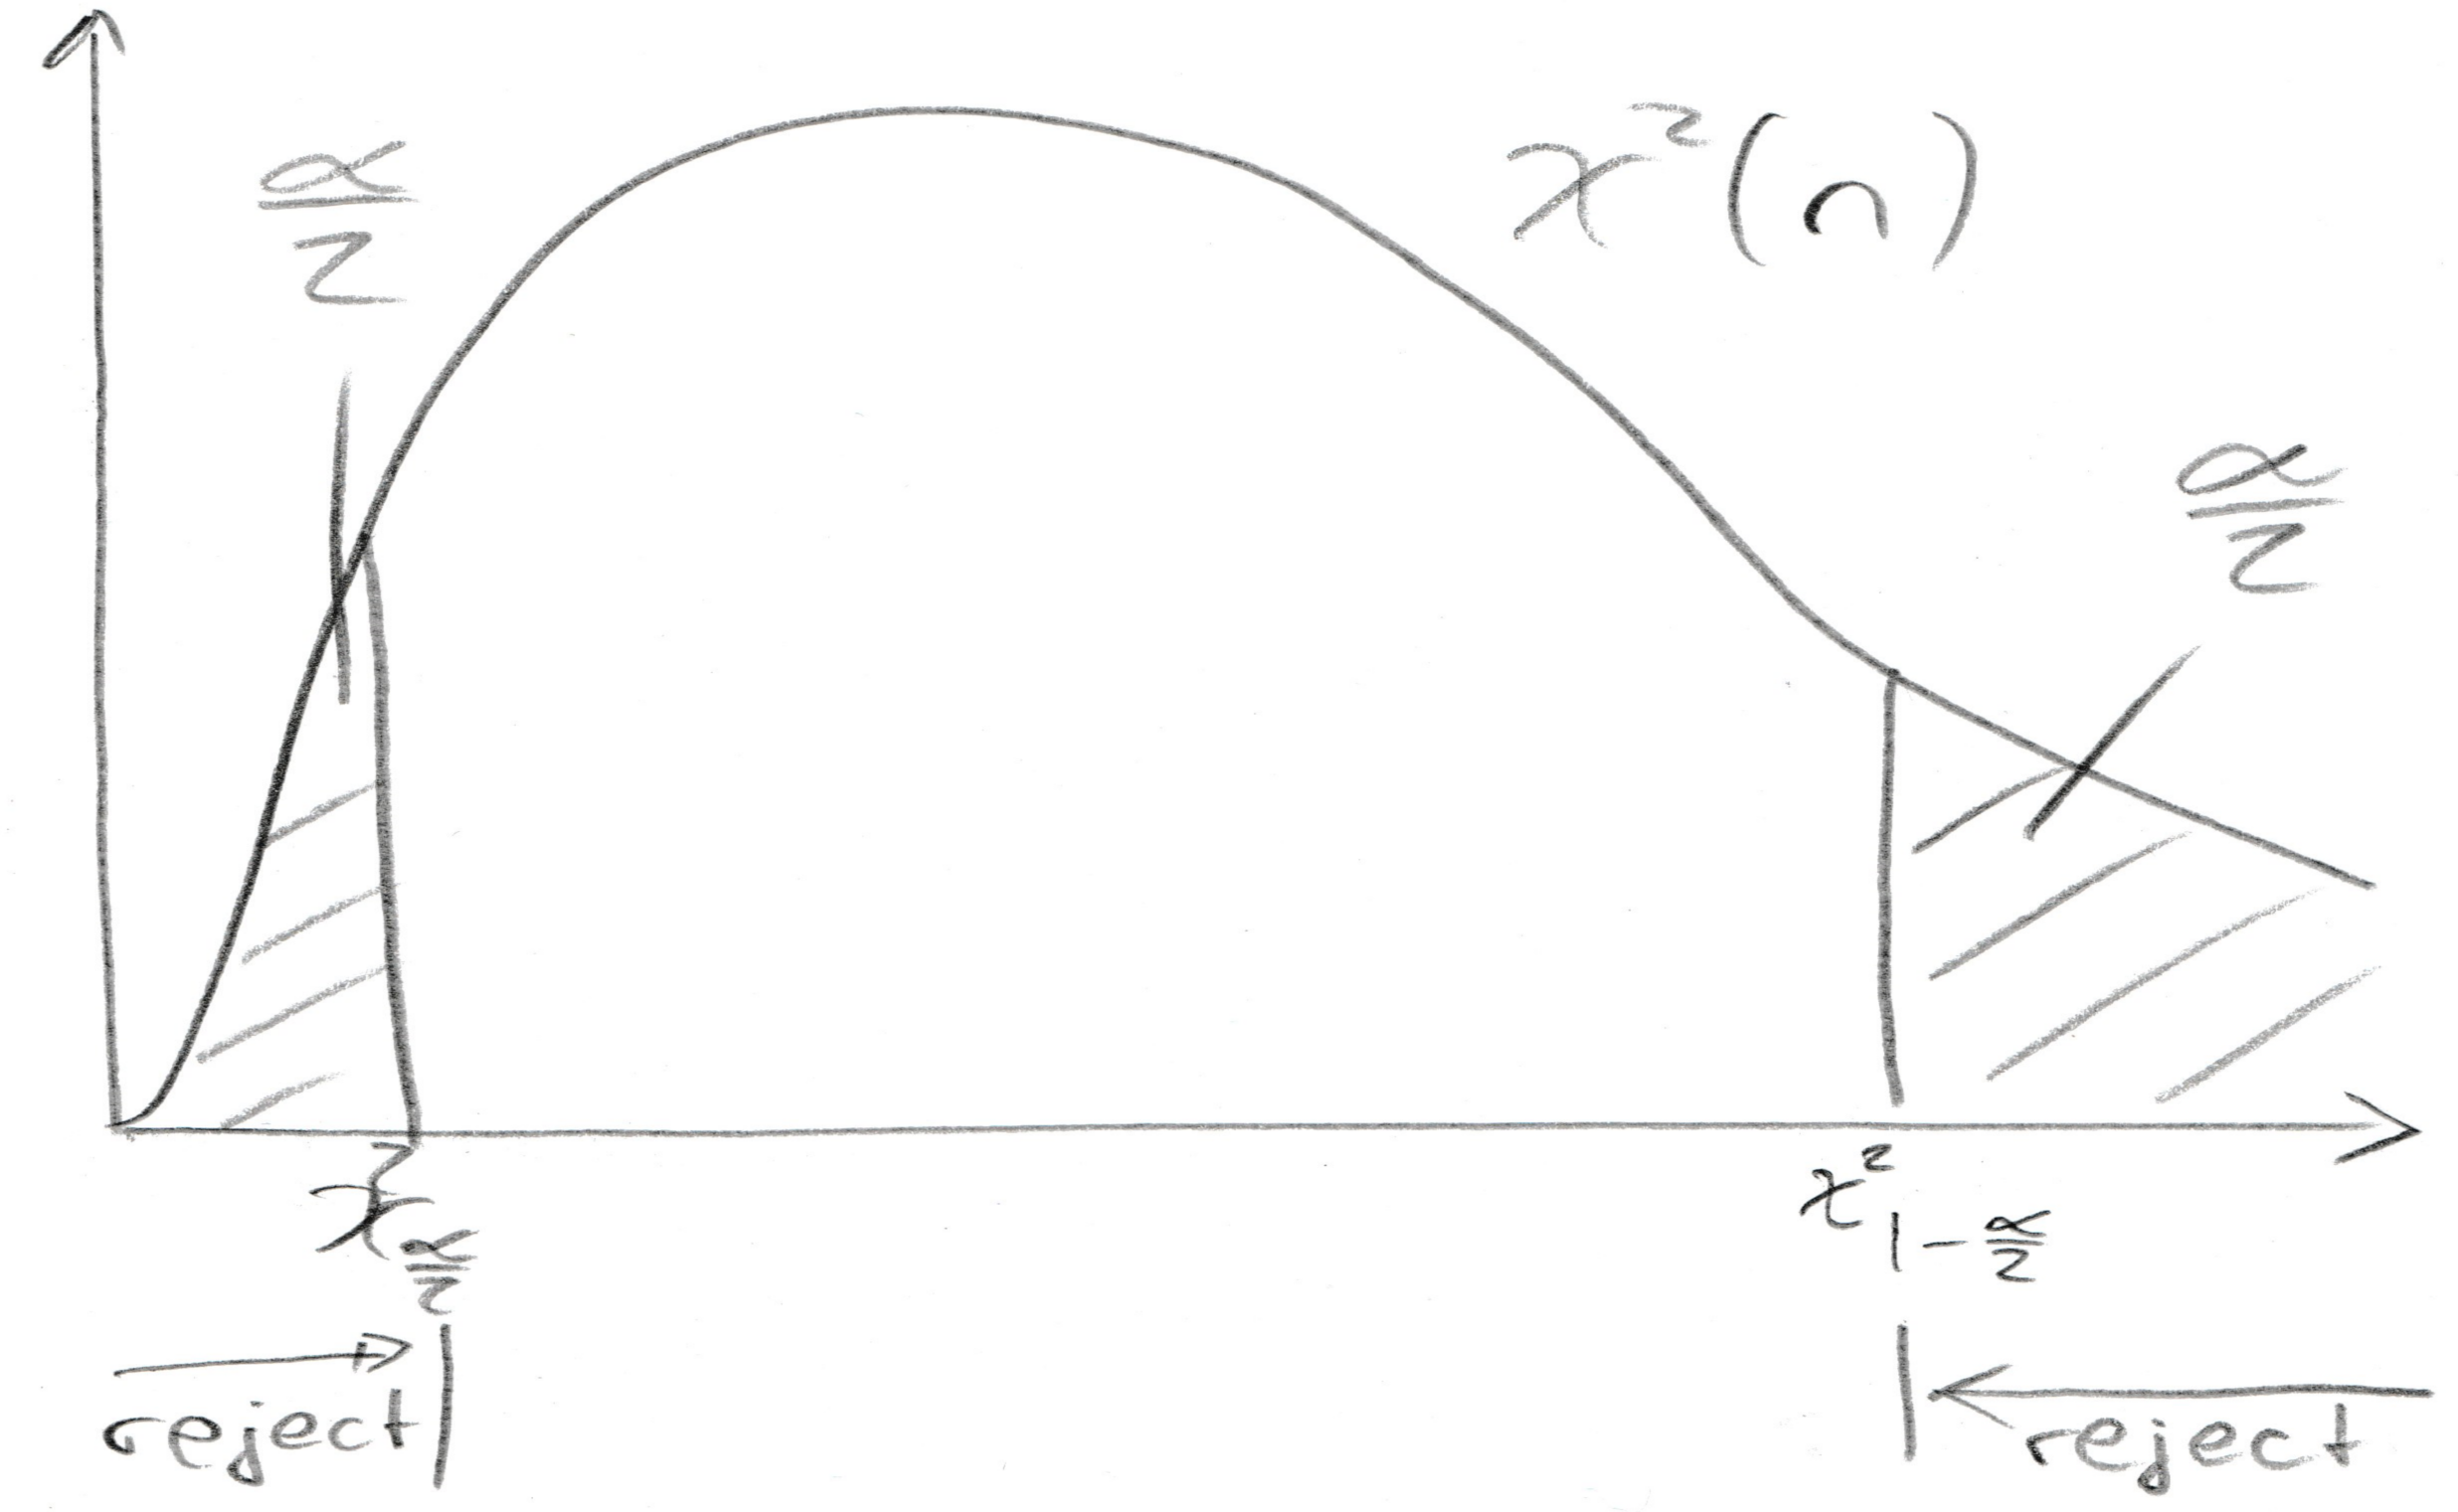
\includegraphics[width=\textwidth]{P14chisq.png}
		\end{fig}			

\subsection{Hypothesis Testing}
	With \emph{hypothesis testing}, we can assess if the value for a parameter we got from an estimator differs from a set value by chance because it is truly different, so it is not related to the actual value of interest. The case of no relation existing is called \emph{null hypothesis}. Hypothesis testing always follows the same framework of the following three steps: 
	\begin{enumerate}
		\item Formulate a null hypothesis $H_0$ and an alternative hypothesis $H_1$ or $H_a$.
		\item Pick a test statistic (a function based on the sample data) which helps to decide between $H_0$ and $H_1$, and gives a distribution if $H_0$.
		\item Calculate the test statistic, pick a probability $\alpha$ of being wrong if $H_0$ is true, \enquote{a burden of proof}. State and apply a decision rule (i.e. a rejection region). Conclude the results clearly.
	\end{enumerate}
	Depending of the question the test is carried out for, $H_0$ can be described with an $=,\,\leq,$ or $\geq$ sign. $H_1$ is the negated version of $H_0$, so not less or equal which means greater than. The mentioned distribution of the test statistic usually will be Normal ($N$), $F(p,q)$ or Chi-Squared ($\chi^2(n)$). The results can either indicate that we have to \emph{reject} $H_0$, or if we cannot confirm that the null hypothesis is wrong, we \emph{fail to reject it}.
	\begin{defi}[Errors in hypothesis testing]{defi:hyperror}
		There are two types of errors which occur when conducting hypothesis testing.
		\centering{
			\begin{tabular}{p{0.2\linewidth}|p{0.35\linewidth}|p{0.35\linewidth}}
				actual truth $\rightarrow$ test result $\downarrow$ & $H_0$ is true & $H_0$ is false\\\hline
				reject $H_0$ & Type I error. Control error size by choosing $\alpha$. & OK\\\hline
				fail to reject $H_0$ & OK & Type II error. $P\sim(E_{II})=\beta$.
			\end{tabular}
		}
	\end{defi}
	\begin{exmp}[Hypothesis statements]{exmp:hypstate}
		We want to asses whether increasing the landing fees at John-Wayne Airport (SNA) has an impact on the number of monthly flights as SNA?
		\begin{enumerate}
			\item $N=\#$flights at SNA. Current $\#$flights is $N_0$.
				\begin{equation*}
					H_0:\;N=N_0\qquad vs. \qquad H_1:\;N\neq N_0
				\end{equation*}
			\item Will a 10\% increase in landing fees show in a decrease in $\#$flights?
				\begin{equation*}
				H_0:\;N\geq N_0\qquad vs. \qquad H_1:\;N<N_0
				\end{equation*}
		\end{enumerate}
	\end{exmp}
	\subsubsection{Interference about a single population}
		We assume that the samples we have come from approximately normal distributed populations. The results are robust against \emph{small} deviations from this assumption in reality.
		\myparagraph{Test a population mean with unknown variance}
			\begin{enumerate}
				\item State $H_0$ and $H_1$ context specific.
				\item Pick the test statistic $T^*=\frac{\bar{x}-\mu_0}{s/\sqrt{n}}$. If $H_0$ is true, $T^*\sim t(n-1)$.
				\item Calculate $T^*$. Pick the confidence level (and probability for a type I error) $\alpha$. Common values for $\alpha$ are 0.5\%, 1\%, 5\%, or 10\%.
			\end{enumerate}
			The idea is to reject $H_0$ if the observation is highly unlikely to be based on this hypothesis.
			\begin{exmp}[One- and two-tailed hypothesis tests]{exmp:tails}
				One-tailed: $H_0:\;\mu=\mu_0\; vs. \; H_1:\;\mu\neq\mu_0$\hfill Two-tailed: $H_0:\;\mu\geq\mu_0\; vs. \; H_1:\;\mu<\mu_0$
				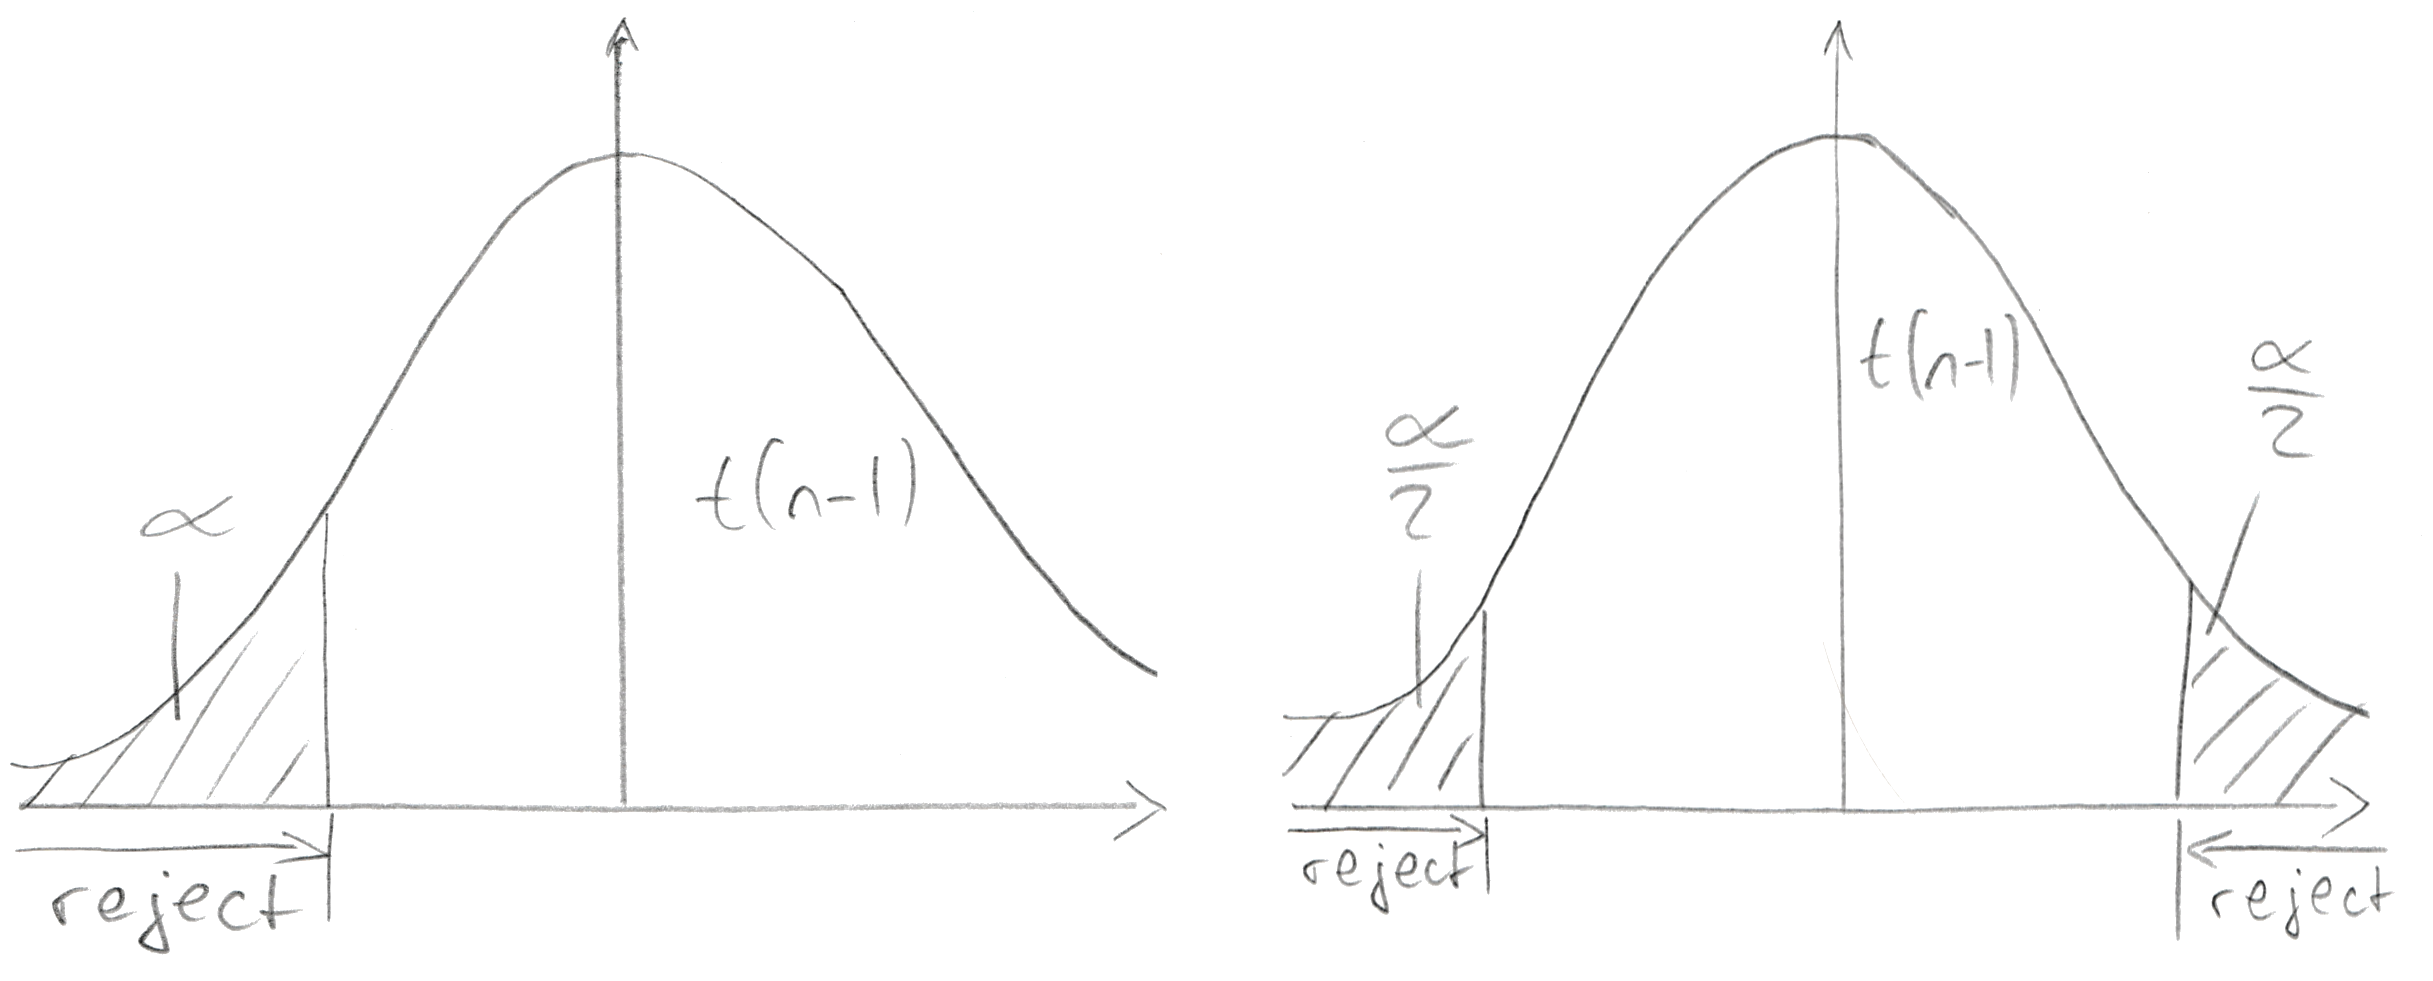
\includegraphics[width=\textwidth]{P15-16-tails.png}
			\end{exmp}
		\myparagraph{Test a population variance}	
			The same 3-step-framework is used. For testing a null hypothesis of $\sigma_0^2$ from a sample size $n$, the test statistic is
			\begin{equation*}
				\chi^2=\frac{(n-1)s^2}{\sigma^2_0}.
			\end{equation*}
			If $H_0$ is true, $\chi^2\sim\chi^2(n-1)$.
			\begin{exmp}[Hypothesis testing for variance]{exmp:vartest}
				Testing if the variance of vehicle speeds on the I-405 on weekday afternoons equal to $10 MPH^2$? We have a random sample with $n=100$ from which we calculate $s^2=9 MPH^2$.
				\begin{enumerate}
					\item $H_0:\;\sigma^2=\sigma^2_0=10 MPH^2 \qquad vs. \qquad H_1\sigma^2\neq 10 MPH^2$
					\item $\chi^2=\frac{(n-1)s^2}{\sigma_0^2},\; \chi^2\sim\chi^2(n-1)$
					\item $\alpha=5\%=0.05,\; \chi^2=\frac{99\cdot9}{10}=89.1$ This value is within the confidence interval of $\left[73.36,128.42\right]$. Therefore, we fail to reject the null hypothesis.
				\end{enumerate}
			\end{exmp}
		\myparagraph{Test a population proportion}	
			We use the same framework to test if a population has a certain proportion $p$. The following $z$ test statistic is used:
			\begin{equation*}
				Z^*=\frac{\hat{p}-p_0}{\sqrt{\frac{\hat{p}(1-\hat{p})}{n}}}\text{. If $H_0$ is true, }z\sim N(0,1)
			\end{equation*}		
			with $\hat{p}$ as a random variable that gives us the sample proportion, $p_0$ as the proportion specified in $H_0$ and sample size $n$.
	\subsubsection{Comparison of two populations}
		\myparagraph{Compare two means from independent samples}	
			Assume that the CLT (\ref{sec:clt}) applies. Using the same framework, we test for the sample means as estimators of the population mean.
			\begin{equation*}
				Z^*=\frac{\bar{x_1}-\bar{x_2}-(\mu_{01}-\mu_{01})}{\sqrt{\frac{s_1^2}{n_1}+\frac{s_2^2}{n_2}}}
			\end{equation*}
			\begin{exmp}[Hypothesis testing average on-time flights]{exmp:meantest}
				We test if \emph{1: Lufthansa} or \emph{2: Air France} is more on time in average. Therefore, we test for $H_0$ of Lufthansa being more on time.
				\begin{equation*}
					H_0:\;\mu_{10}-\mu_{20}\leq 0\qquad vs. \qquad H_1:\;\mu_1-\mu_2>0
				\end{equation*}
			\end{exmp}
			If $H_0$ is true, for normal and small samples $n_1,n_2\leq 25$, $T\sim t_{dof}$ with $dof$ degrees of freedom (rounded to the next integer).
			\begin{equation*}
				dof=INT\left[\frac{\left(\frac{s_1^2}{n_1}+\frac{s_2^2}{n_2}\right)^2}{\frac{(s_1^2/n_1)^2}{n_1-1}+\frac{(s_2^2/n_2)^2}{n_2-1}}\right]
			\end{equation*}	
			If the populations have the same variances, the following test statistic can be used and compared to a t-distribution with $dof=n_1+n_2-2$.
			\begin{equation*}
				\frac{\bar{x_1}-\bar{x_2}-(\mu_{10}-\mu_{20})}{\sqrt{s^2\left(\frac{1}{n_1}+\frac{1}{n_2}\right)}}
			\end{equation*}
		\myparagraph{Compare two means from paired observations}	
			For two paired datasets of the size $n_d$ and the difference parameters marked by $\bar{x_d},s_d$, we use the following test statistic:
			\begin{equation*}
				T^*=\frac{\bar{x_d}\mu_0}{s_d/\sqrt{n_d}}\text{. If $H_0$ is true, }T^*\sim t(n_d-1)
			\end{equation*}				
		\myparagraph{Evaluate the difference between two population proportions}	
			For large enough sample size, we can test differences as $H_0:\;p_1-p_2=,\leq,\geq p_{d0}$.
			\begin{equation*}
					Z^*=\frac{\hat{p}_1-\hat{p}_2-p_d}{\sqrt{\frac{\hat{p}_1(1-\hat{p}_2)}{n_1}+\frac{\hat{p}_1(1-\hat{p}_2)}{n_2}}}\text{. If $H_0$ is true, }Z^*\sim N(0,1)				
			\end{equation*}
		\myparagraph{Compare two population variances}
			They can be compared using the following f-test:	
			\begin{equation*}
				F^*=\frac{s_1^2}{s_2^2}\text{. If $H_0$ is true, }F^*\sim F(n_1-1,n_2-1)				
			\end{equation*}
		Further information on hypothesis testing can be found in \textcite{Conover.1999} and \textcite[p. 28ff.]{Washington.2011}.		
\begin{famo}[Karl Pearson]{famo:pearson}
		\emph{Karl Pearson} (March 1857 – 27 April 1936) was an English mathematician and biostatistician. He established the discipline of mathematical statistics, and contributed significantly to biometrics, meteorology. Pearson was a protégé and biographer of Sir Francis Galton, who coined the term \enquote{regression}.
	
	After a private education at University College School, he went to King's College, Cambridge in 1876 to study mathematics. He then traveled to Germany to study physics and metaphysics in Heidelberg. He attended lectures on Darwinism, but also Roman law, medieval and 16th century German literature, and Socialism in Berlin.
	
	After returning to London, he studied law until 1881 but never practiced. He then returned to mathematics, first at King's College, London in 1881 and then at University College, London in 1883. After his appointment to the professorship of Geometry at Gresham College, he met Walter Frank Raphael Weldon, a zoologist with whom he developed a fruitful collaboration. Weldon introduced him to Darwin's cousin Francis Galton. Pearson became Galton's protégé, and after Galton's death in 1911, he wrote his biography. He formed the Department of Applied Statistics, into which he incorporated the Biometric and Galton laboratories. In 1890, he married Maria Sharpe, and they had three children. 
	
	Unfortunately, Pearson was racist, anti‐Semitic, and a proponent of eugenics, i.e., a social philosophy advocating the improvement of human genetic traits through the promotion of higher rates of reproduction for people with desired traits, and reduced rates of reproduction and sterilization of people with less‐desired or undesired traits. 

	Pearson's work embraced wide applications and the development of mathematical statistics, with contributions to \emph{biology, epidemiology, anthropometry, medicine, psychology and social history}. In 1901, with Weldon and Galton, he founded the journal Biometrika that focuses on statistical theory. Pearson's thinking underpins many of the 'classical' methods which are in common use today. Some contributions are:
	\begin{itemize}
		\setlength{\itemsep}{0pt}
		\setlength{\parskip}{0pt} 		
		\item Correlation coefficient. He studied its relationship with  linear regression,
		\item method of moments: Pearson introduced the concept borrowed from physics,
		\item Pearson's system of continuous univariate probability distributions that came to form the basis of the now conventional continuous probability distributions,
		\item foundations of hypothesis testing and of the statistical decision theory,
		\item use of P-values and Pearson's chi-squared test,
		\item Principal component analysis. 
	\end{itemize}
	\credits{Source: \url{https://en.wikipedia.org/wiki/Karl_Pearson}}
\end{famo}			